 \documentclass{beamer}
\usepackage{physics,tikz,amsmath,amsfonts,amssymb,amsthm,multirow,slashed,graphicx,relsize,biblatex}
 \usepackage[compat=1.1.0]{tikz-feynman}
\setlength{\unitlength}{1mm}
\addbibresource{cite.bib}
\newcommand{\nn}{\nonumber}
\usetheme{Boadilla}
\definecolor{lavenderblush}{rgb}{1.0, 0.94, 0.96}
\definecolor{1}{HTML}{1F4C34}
\definecolor{beamer@barcolor}{RGB}{194,193,204}
\definecolor{beamer@normaltextcolor}{RGB}{84,97,110}
\definecolor{beamer@headercolor}{rgb}{0,0.41,0.54} 
\setbeamercolor{structure}{fg=1}
\setbeamercolor{normal text}{fg=beamer@normaltextcolor}
\setbeamercolor{frametitle}{fg=lavenderblush,bg=1}
\setbeamercolor{Feather}{fg=beamer@barcolor,bg=beamer@headercolor}
\title[$e^++e^-\rightarrow Z + H$]{$Zh$ production at lepton collider}
\author{Lê Văn Dũng}
\institute[HCMUS]{Ho Chi Minh City University of Science\\
       Department of Theoretical Physics}
\date{\today}
\begin{document}
\begin{frame}
\titlepage
\end{frame}
\begin{frame}{Table of Contents}
    \tableofcontents
\end{frame}
\section{Scattering process in the Standard Model}
\begin{frame}
\frametitle{Feynman rules}
The Feynman diagram that associates with the process $e^++e^-\rightarrow Z + h$ is
\begin{align*}
&\feynmandiagram [medium, horizontal=b to d] {
a [label=$e^-$] -- [fermion] b -- [fermion] c[label=$e^+$],
b -- [boson,edge label =$Z$] d,
e[label=$Z$] -- [boson] d -- [scalar] f[label=$h$]
};
\end{align*}
\end{frame}
\begin{frame}
\frametitle{Feynman rules}
Lagrangian of Standard model
\begin{align*}
\mathcal{L}_{SM}=\mathcal{L}_{Fermion}+\mathcal{L}_{gauge}+\mathcal{L}_{Higgs}+\mathcal{L}_{Yukawa}.
\end{align*}

The Fermion Lagrangian
\begin{align*}
\mathcal{L}_{Fermion}=   i\overline{\psi}(x) \gamma^\mu D_\mu \psi(x).
\end{align*}
is the $gauge$ $invariant$ kinetic term of fermion fields where gauge fields $A_\mu,Z_\mu,W^\pm_\mu$ are introduced as a \textbf{connection} between field values at different points in space.
\begin{align*}
\feynmandiagram [inline=(a.base),horizontal=a to b] {
  i1 [particle=$e^-$] -- [fermion] a -- [fermion] i2 [particle =$e^+$],
  a -- [photon] b [particle=$Z$],
};
=& \frac{ig}{2\cos_w} \frac{\gamma^\mu(1-4 \sin^2\theta_W+\gamma^5)}{2}
\end{align*}
\end{frame}
\begin{frame}
\frametitle{Feynman rules}
\begin{align*}
\mathcal{L}_{gauge}=-\frac{1}{4} F_{\mu\nu}F^{\mu\nu},
\end{align*}
gauge invariant kinetic term for the gauge field
\begin{align*}
\mathcal{L}_{Higgs}=(D_\mu\phi)^\dagger D^\mu \phi - V(\phi),
\end{align*}
kinetic term of scalar field, responsible for spontaneous symmetry breaking.
\begin{align*}
    \feynmandiagram [inline=(a.base),medium, horizontal=a to b]{
    a [dot] -- [boson,edge label'=\(Z\),momentum=$q$ ] b [dot]
    };&=\frac{-i}{q^2-m_Z^2+i\epsilon}\left(g_{\mu \nu}-\frac{q_\mu q_\nu}{q^2-\xi m^2_Z}(1-\xi)\right),\\
         \feynmandiagram[inline=(a.base),medium, horizontal=a to b]{
    a [dot] -- [scalar ] b 
    };&=1.\\
    \feynmandiagram [inline=(d.base),small,horizontal=b to d] {
a [particle=\(Z\)]  -- [boson] b -- [boson] c[particle =\(Z\)],
b -- [scalar] d [particle=\(h\)],
};
&=\ 2i\frac{g^{\mu\nu}}{v}m_Z^2
\end{align*}
\end{frame}
\begin{frame}
\frametitle{Feynman rules}
\begin{align*}
\mathcal{L}_{Yukawa}=-G_l^{ij}\overline{L}^{i}_L\phi l^{j}_R\ \subset -m_e \overline{e}e,
\end{align*}
responsible for generating the mass term of the fermions, after symmetry have been broken.\\
combine with kinetic term, we now can write down Feynman rules for the fermion
\begin{align*}
    \feynmandiagram[inline=(a.base),medium, horizontal=a to b]{
    a  -- [fermion, momentum=\(p\) ] b [dot]
    };&=u^s(p),\\
     \feynmandiagram[inline=(a.base),medium, horizontal=a to b]{
    a  --  [anti fermion, momentum=\(p\) ]  b [dot]
    };&=\overline{v}^s(p).
\end{align*}
\end{frame}
\begin{frame}
\frametitle{Cross-section in the Standard Model}
\centering
	\begin{picture}(100,65)
    \put(50,0){$E_{CM}$(GeV)}
    \put(-7,40){$\sigma$(fb)}
    \put(0,5){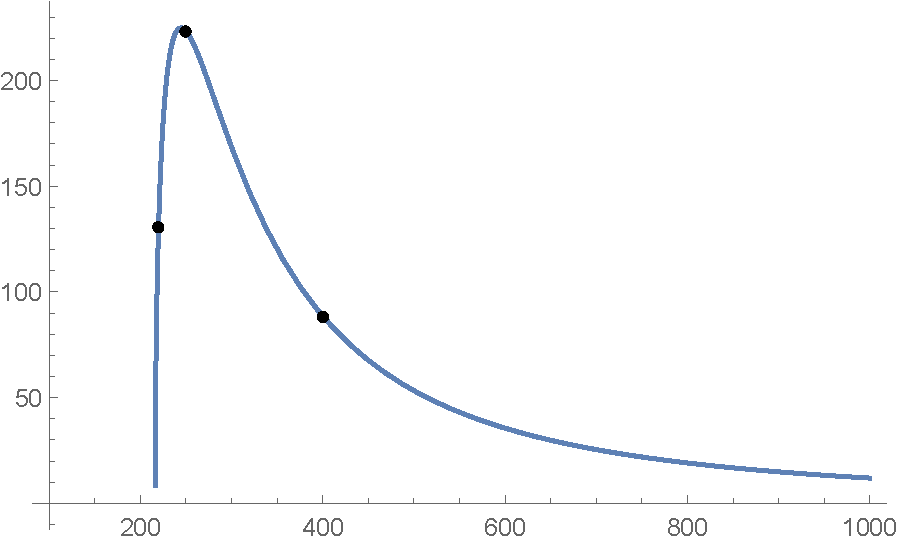
\includegraphics[scale=0.7]{SMscatter.pdf}}
    \end{picture}
Total cross-section of $e^+e^- \rightarrow Zh$ in SM\\
$m_Z+m_h\approx 216 (GeV)$
\end{frame}
\begin{frame}
\frametitle{Cross-section in the Standard Model}
\hspace{1cm}\begin{picture}(100,65)
    \put(50,0){$\theta$ (Rad)}
    \put(-7,40){$\frac{d\sigma}{\cos \theta}$(fb)}
    \put(0,5){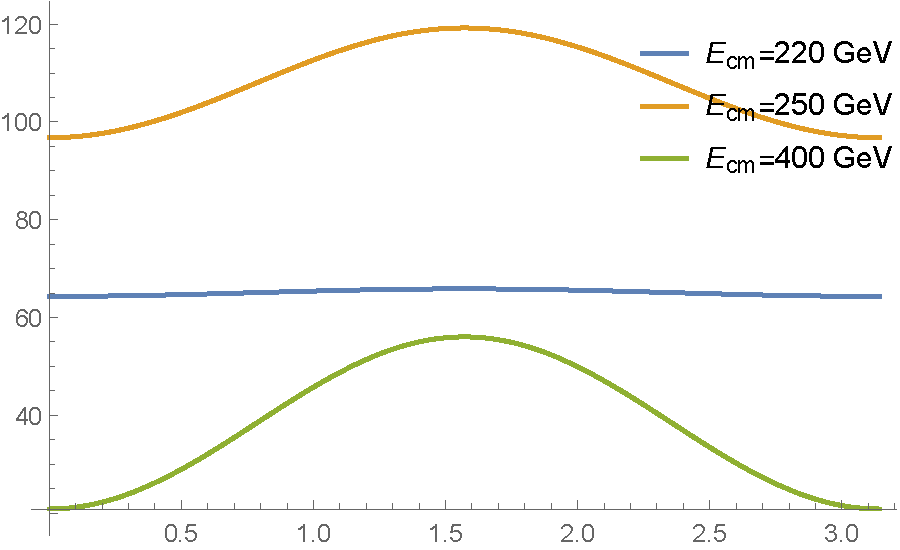
\includegraphics[scale=0.7]{diff-cross.pdf}}
    \end{picture}\\
differential cross-section of $e^+e^- \rightarrow ZH$ at $E_{CM}=220,250,400$ GeV 
\end{frame}
\section{scattering process in the extended $U(1)_{B-L}$ model}
\begin{frame}
\frametitle{Extended $U(1)_{B-L}$ model}
Normally, symmetry of a classical theory is also a symmetry of the quantum theory. But sometimes, it is not.\\
Requirement of $U(1)_Y$ hypercharges for our SM to be \textbf{anomaly free}.
\begin{align*}
\partial_\mu J_Y^\mu \thicksim(2Y^3_L-Y_e^3-Y_\nu^3) + 3 (2Y^3_Q-Y_u^3-Y_d^3)=0.
\end{align*}
substitute
\begin{align*}
Y_L=-\frac{1}{2},\quad Y_e=-1, \quad Y_\nu=0,\quad  Y_Q=\frac{1}{6},\quad Y_u=\frac{2}{3},\quad Y_d=-\frac{1}{3},
\end{align*}
we have 
\begin{align*}
0=\frac{3}{4}-\frac{3}{4}.
\end{align*}
The anomaly vanishes for any generation of fermion, but won't vanish for quark or lepton alone.
\end{frame}
\begin{frame}
\frametitle{Extended $U(1)_{B-L}$ model}
Does there exist another $U(1)$ gauge group
\begin{align*}
SU(3)_C\times SU(2)L \times U(1)_Y\times U(1)_{Y'}
\end{align*}
Yes there is, and the $U(1)_{Y'}$ charges are
\begin{align*}
Y_L'=Y_{e_R}'=Y_{\nu_R}'=-1, \quad Y_Q'=Y_{u_R}'=Y_{d_R}'=\frac{1}{3},
\end{align*}
The new charges for fermions are exactly the baryon minus lepton number, therefore the new gauge group is called $U(1)_{B-L}$. You can see that \textbf{right-handed neutrinos} does have a charge in the new gauge group so their existence in this model is real.
\end{frame}
\begin{frame}
\frametitle{Extended $U(1)_{B-L}$ model}
\begin{align*}
D_\mu&=\partial_\mu - ig_s \frac{\lambda^a}{2}G_\mu^a-i g I^a W_\mu^a-i g' YB_\mu -i(\tilde{g} Y+ g_1' Y_{B-L})B_\mu'\\
\end{align*}
\begin{align*}
&\mathcal{L}_{fermion}&&=\mathcal{L}_{SM}+ i\overline{\nu}_R \gamma^\mu D_\mu \nu_R\\\\
&\mathcal{L}_{gauge}&&=\mathcal{L}_{SM}+ \frac{1}{4}F'_{\mu\nu}F'^{\mu\nu}\\\\
&\mathcal{L}_{Yukawa}&&=\mathcal{L}_{SM}-G^{ij}_\nu\overline{L}^{i}_L \phi^c \nu_R^{j}-
G_M\overline{\nu_R^c}^{i} \chi\nu_R^{j}+h.c\\\\
&\mathcal{L}_{Higgs}&&=\mathcal{L}_{SM}+(D^\mu\chi)^\dagger  D_\mu \chi- V(H,\chi)\\
&V(H,\chi)&&=	m^2|H|^2+\mu^2|\chi|^2+\begin{pmatrix}
|H|^2 & |\chi|^2
\end{pmatrix}
\begin{pmatrix}
\lambda_1 & \frac{\lambda_3}{2}\\
\frac{\lambda_3}{2}& \lambda_2
\end{pmatrix}
\begin{pmatrix}
|H|^2\\
|\chi|^2
\end{pmatrix}
\end{align*}
\end{frame}
\begin{frame}
\frametitle{Extended $U(1)_{B-L}$ model}
\center{\textbf{Higgs sector}}\\
The fields configuration that minimize the vaccum $V(H,\chi)$ is
\begin{align*}
\langle H\rangle=\frac{1}{\sqrt{2}}\begin{pmatrix}
0\\v
\end{pmatrix},&& \langle \chi\rangle =\frac{x}{\sqrt{2}}
\end{align*}
$x$ is suppose to have the value at the scale of  \textbf{TeV}
because it give mass to $Z'$ and it's mass should be higher than what we can measure currently.\\
Using the freedom of gauge transformation to set the field to unitary gauge
\begin{align*}
H=\frac{1}{\sqrt{2}}\begin{pmatrix}
0\\
v +h
\end{pmatrix},&&\chi=\frac{1}{\sqrt{2}}(x+h') .
\end{align*}
\end{frame}
\begin{frame}
\frametitle{Extended $U(1)_{B-L}$ model}
Expanding Higgs kinetic terms
\begin{align*}
 (D^\mu H)^\dagger  D_\mu H+(D^\mu\chi)^\dagger  D_\mu \chi
\end{align*}
\begin{align*}
\frac{1}{2}\left(\frac{v}{2}\right)^2 \begin{pmatrix}
W^3& B_\mu & B'_\mu
\end{pmatrix}\begin{pmatrix}
g^2& -g g'& -g \tilde{g}\\
-g g'&g'^2& g' \tilde{g}\\
-g \tilde{g}& g' \tilde{g} &\tilde{g}^2+ 16 g_1'^2\left(\frac{x}{v}\right)^2
\end{pmatrix}\begin{pmatrix}
W^3\\ B_\mu \\ B'_\mu
\end{pmatrix},
\end{align*}
diagonalizing the mass matrix return us with 3 eigen-masses, one of which is 0.
When they decouple, we are returned with our Standard Model masses
\begin{align*}
m_A&=0,\\
m_Z&=\frac{1}{2}\sqrt{g^2+g'}\\ 
m_{Z'}&=2 g_1' x
\end{align*}
\end{frame}
\begin{frame}
\frametitle{Extended $U(1)_{B-L}$ model}
Higgs fields also got mixed, after unmix them, we have
\begin{align*}
m_{h_1}^2=\lambda_1 v^2+\lambda_2 x^2-\sqrt{(\lambda_1 v^2-\lambda_2 x^2)^2+(\lambda_3 x v)^2}\\
m_{h_2}^2=\lambda_1 v^2+\lambda_2 x^2+\sqrt{(\lambda_1 v^2-\lambda_2 x^2)^2+(\lambda_3 x v)^2},
\end{align*}
the lighter one is considered as our good old SM Higg, and the heavier one will be the new higgs, which doesn's interact with normal SM particle. We are free to set 
\begin{equation}
m_{h_1}=m_h (SM)\nn
\end{equation}
\end{frame}
\begin{frame}
\frametitle{Basic diagram}
\begin{align}
&\feynmandiagram [medium, horizontal=b to d] {
a [label=$e^-$] -- [fermion] b -- [fermion] c[label=$e^+$],
b -- [boson,edge label =$Z$] d,
e[label=$Z$] -- [boson] d -- [scalar] f[label=$h$]
};,&&\quad
\feynmandiagram [medium, horizontal=b to d] {
a [label=$e^-$] -- [fermion] b -- [fermion] c[label=$e^+$],
b -- [boson,edge label =$Z'$] d,
e[label=$Z$] -- [boson] d -- [scalar] f[label=$h$]
};\nn\\
&\qquad\qquad\qquad M_1 &&\qquad\qquad\qquad M_2\nn
\end{align}
\end{frame}
\begin{frame}
\frametitle{Basic diagram}
Working out the Feynman rules for the vetices is self explanatory.\
Now I present you some of the basic decaying width of the $Z'$ that will be used for the calculation the scattering process.
\begin{align*}
\feynmandiagram [medium, horizontal=b to d] {
b[label=$Z'$] -- [boson,momentum=$p_1$] d,
e[label=$\overline{f}$] -- [fermion,rmomentum'=$p_3$] d -- [fermion,momentum=$p_2$] f[label=$f$]
};
\end{align*}
\begin{align*}
\mathcal{M}=\overline{u}(p_2) \lambda_{ffZ'}\gamma^\mu(g_A'-g_V' \gamma^5) v(p_3) \epsilon_\mu(p_1),
\end{align*}
\end{frame}

\begin{frame}\frametitle{Basic diagram}

\begin{align*}
&\feynmandiagram [small, horizontal=b to d] {
b[label=$Z'$] -- [boson,momentum=$p_1$] d,
e[label=$Z$] -- [boson,rmomentum'=$p_2$] d -- [scalar,momentum=$p_3$] f[label=$h$]
};&\mathcal{M}&=\lambda_{ZZ'h} \epsilon_\mu^*(p_1)g^{\mu\nu} \epsilon_\nu^*(p_2)
\end{align*}
\begin{align*}
\feynmandiagram [small, horizontal=b to d] {
b[label=$Z'_\mu$] -- [boson,momentum=$p_1$] d,
e[label=$W^+_\nu$] -- [boson,rmomentum'=$p_2$] d -- [boson,momentum=$p_3$] f[label=$W^-_\lambda$]
};
\end{align*}
\begin{align*}
\mathcal{M}&=i g c_w \sin(\phi_{BL})\left[g_{\mu\nu}(p_1-p_2)_\lambda+g_{\nu\lambda}(-p_2+p_3)_\mu+g_{\lambda\mu}(-p_3-p_1)_\nu\right],
\end{align*}
\end{frame}
\begin{frame}
\frametitle{Total decay width of $Z'$}
  \hspace{1.5cm} \begin{picture}(100,60)
    \put(50,0){$m_{Z'}$(GeV)}
    \put(-15,40){$\Gamma_{Z'}$ (GeV)}
    \put(0,5){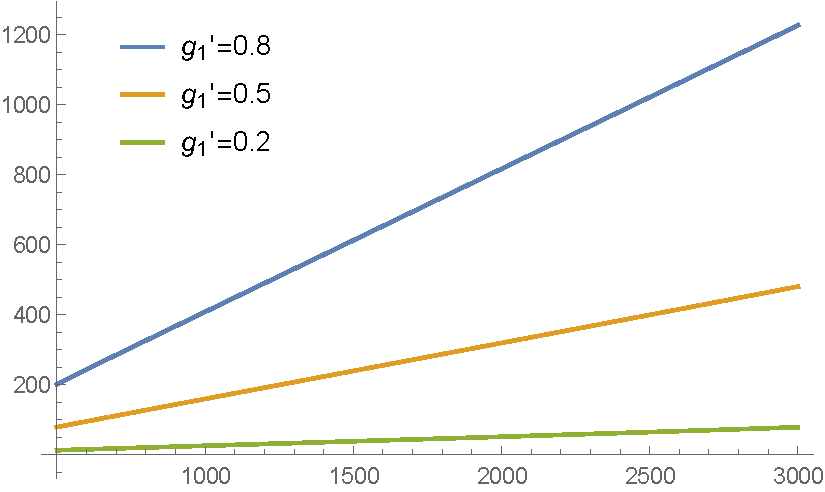
\includegraphics[scale=0.7]{mZ-decay.pdf}}
    \end{picture}\\
\begin{center}
Total decay width of $Z'$ for different B-L coupling parameters $g_1'$
\end{center}
\end{frame}
\begin{frame}
\frametitle{Total decay width of $Z'$}
   \begin{center}
    \begin{picture}(100,60)
    \put(50,0){$m_{Z'}$(GeV)}
    \put(-10,40){BR}
    \put(71,22){$Z'\rightarrow \overline{f}f $}
    \put(71,12){$Z'\rightarrow W^\pm$}
    \put(71,17){$Z'\rightarrow ZH$}
    \put(0,5){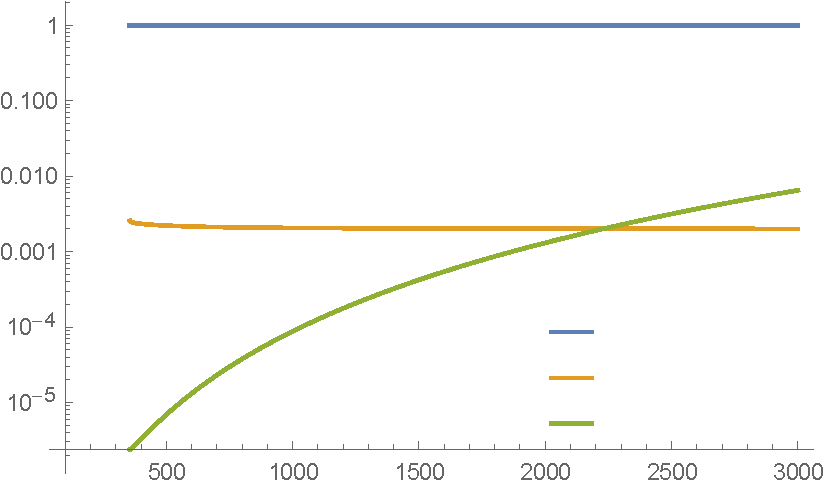
\includegraphics[scale=0.7]{BR}}
    \end{picture}
   \end{center}
\begin{center}
Branching ratio of $Z'$ decay
\end{center}
\end{frame}
\begin{frame}
\frametitle{Cross-section in the $U(1)_{B-L}$ model}
\begin{center}
\begin{picture}(100,60)
    \put(50,0){$E_{CM}$(GeV)}
    \put(-7,40){$\sigma$(fb)}
    \put(0,5){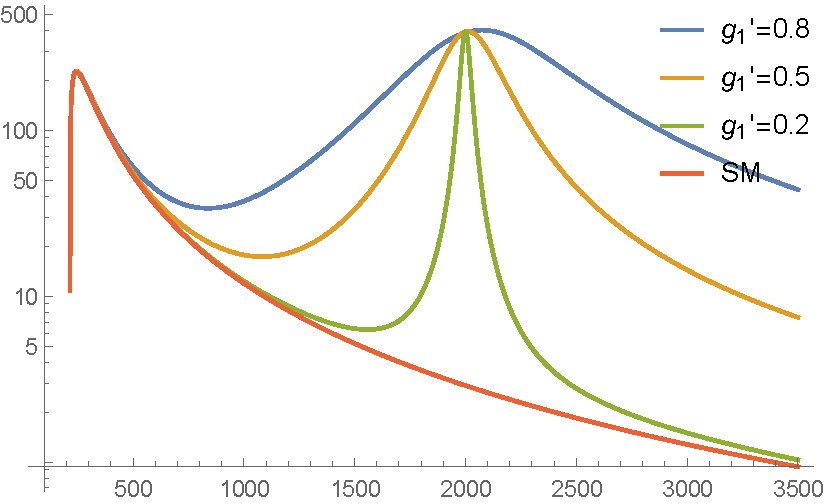
\includegraphics[scale=0.7]{gg.pdf}}
    \end{picture}
\end{center}
\begin{center}
   Cross-section for different B-L coupling parameters $g_1'$ and the classic SM cross-section with $m_{Z'}=2000 GeV$
\end{center}
\end{frame}
\begin{frame}
\frametitle{Cross-section in the $U(1)_{B-L}$ model}
\hspace{1.5cm}\begin{picture}(100,65)
    \put(50,0){$E_{CM}$(GeV)}
    \put(-7,40){$\sigma$(fb)}
    \put(0,5){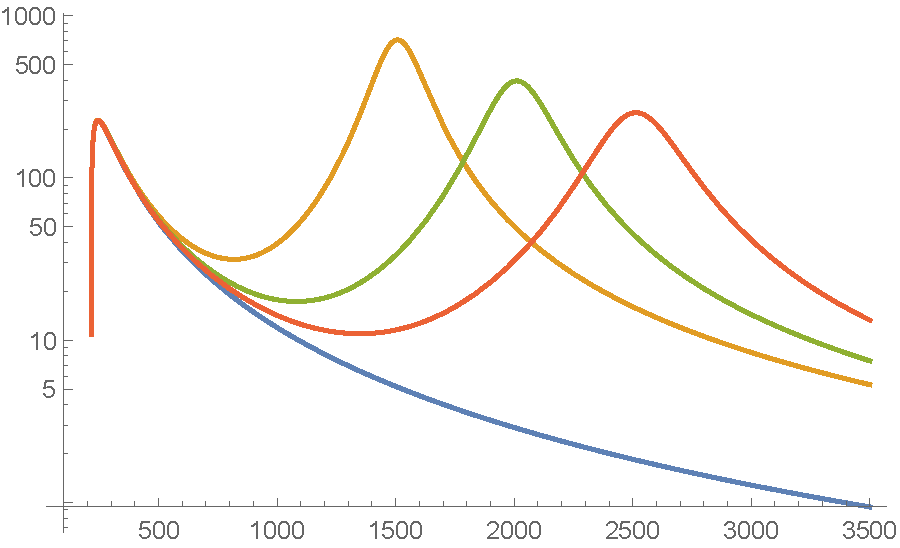
\includegraphics[scale=0.65]{mZ.pdf}}
    \put(20,60){$\phi_{BL}=10^{-3}$}
    \end{picture}
\begin{center}
Cross-section for different $M_{Z'}$ masses $m_{Z'}=1500,2000,2500$ (GeV) and the classic SM cross-section
\end{center}
\end{frame}
\begin{frame}{Reference}
\nocite{davidtong:quantumfieldtheory}
\nocite{Schwartz:2014sze}
\nocite{Basso:2011hn}
\printbibliography
\end{frame}
\begin{frame}
\begin{center}
    \begin{huge}  
 \textbf{ Thank you for listening!} 
\end{huge}  
\end{center}
\end{frame}
\end{document}
